\documentclass[tikz,border=0pt]{standalone}
\usepackage{amsmath}
\definecolor{bgr}{RGB}{40, 126,182}
\usepackage{pgf}
\usepackage{tikz}
\usetikzlibrary{arrows, automata, backgrounds}
\usepackage[latin1]{inputenc}
\begin{document}
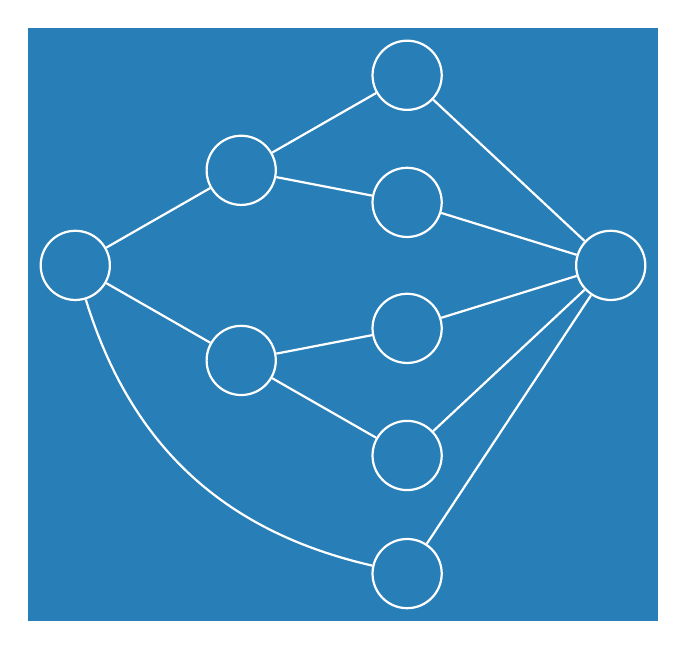
\begin{tikzpicture}[-, node distance=1.cm, thick, inner sep=0pt, background rectangle/.style={fill=bgr}, show background rectangle]
  \node[state, draw=white]  (X)  {};
  \node[state, draw=white]  (X_1) [above right of=X, xshift=1.4cm, yshift=0.5cm]  {};
  \node[state, draw=white]  (X_2) [below right of=X, xshift=1.4cm, yshift=-0.5cm] {};
  \node[state, draw=white]  (P_1) [above right of=X_1, xshift=1.4cm, yshift=0.5cm] {};
  \node[state, draw=white]  (P_2) [below right of=X_1, xshift=1.4cm, yshift=0.3cm] {};
  \node[state, draw=white]  (P_3) [above right of=X_2, xshift=1.4cm, yshift=-0.3cm] {};
  \node[state, draw=white]  (P_4) [below right of=X_2, xshift=1.4cm, yshift=-0.5cm] {};
  \node[state, draw=white]  (P_S) [below of=P_4, yshift=-0.5cm] {};
  \node[state, draw=white]  (Y)   [right of=X, node distance=6.8cm]{};
  \path (X) edge [white]  (X_1)
        (X) edge [white]  (X_2)
        (X) edge [bend right, white] (P_S)
        (X_1) edge [white]  (P_1)
        (X_1) edge [white]  (P_2)
        (X_2) edge [white]  (P_3)
        (X_2) edge [white]  (P_4)
        (P_1) edge [white]  (Y)
        (P_2) edge [white]  (Y)
        (P_3) edge [white]  (Y)
        (P_4) edge [white]  (Y)
        (P_S) edge [white]  (Y)
        ;
\end{tikzpicture}
\end{document}
